\chapter{Method}\label{cha:intro}

\section{Data sets}


\section{Detection and segmentation}

\subsection{Image preprocessing}

\subsection{Heatmap}



\section{Data gathering}\label{sec:research:history}
The GNU Image Manipulation Program, or GIMP, is used for extracting images of cells for training the neural network. However, the blood smear images are too large to handle, so before extracting these cell images the blood smear image is split into smaller files with a size of 2048 by 2048 pixels. Some of these images are chosen in accordance with the method described in 1.5.3. These smaller images are then opened in The GIMP, where a new layer is added, and squares of different colors representing the different cell types are drawn on top of the cells. When all white blood cells have been covered with a square of the corresponding color, the layer with the squares is saved as a PNG image. A simple python script then reads both of these images, and uses the coordinates of the squares to cut out the cells from the cell image and saves them as a sequence of PNG images with the naming convention celltype\_number.png, e.g. lymphocyte\_1.png, lymphocyte\_2.png, ..., lymphocyte\_n.png.

\section{Implementation}\label{sec:research:history}

\subsection{Neural network structure}\label{sec:research:history}

\subsection{Framework}\label{sec:research:history}
The implementation is done in Theano and Lasagne for the Convolutional Neural Network in Python, with additional libraries simplifying and greatly reducing computation time, most notably NumPy for efficient array computations. 

\subsection{Preprocessing}\label{sec:research:history}

\section{Graphical User Interface}
Since this thesis aims to create a semi-automatic method for obtaining an HL ratio, an easy to use GUI must be included. This section details the design and implementation of this interface.

\subsection{Design}
The GUI consists of two main windows, where the first consists of an image viewer that supports zooming in and out of the blood smear image, and the drawing of ROIs. When the user is satisfied with the selected ROIs and clicks on the button labeled "Run", the main algorithm that finds the heterophils and lymphocytes is run, which may take several minutes up to hours, depending on the size of the selected ROIs. When the algorithm is done, the second main window pops up, which shows a grid of nine cells, with left and right buttons to show the next and previous cells found. In this window, it is also possible to show only one type of cell, or choose between the ROIs created. In the upper left corner, the HL ratio for the currently chosen ROI(s) is shown. By right-clicking on the cells in the grid, it is possible to remove or move cells to another category, for example if a lymphocyte is wrongly classified as a heterophil. This feature can be seen in figure XXXXX.

\begin{figure}[h!]
    \centering
    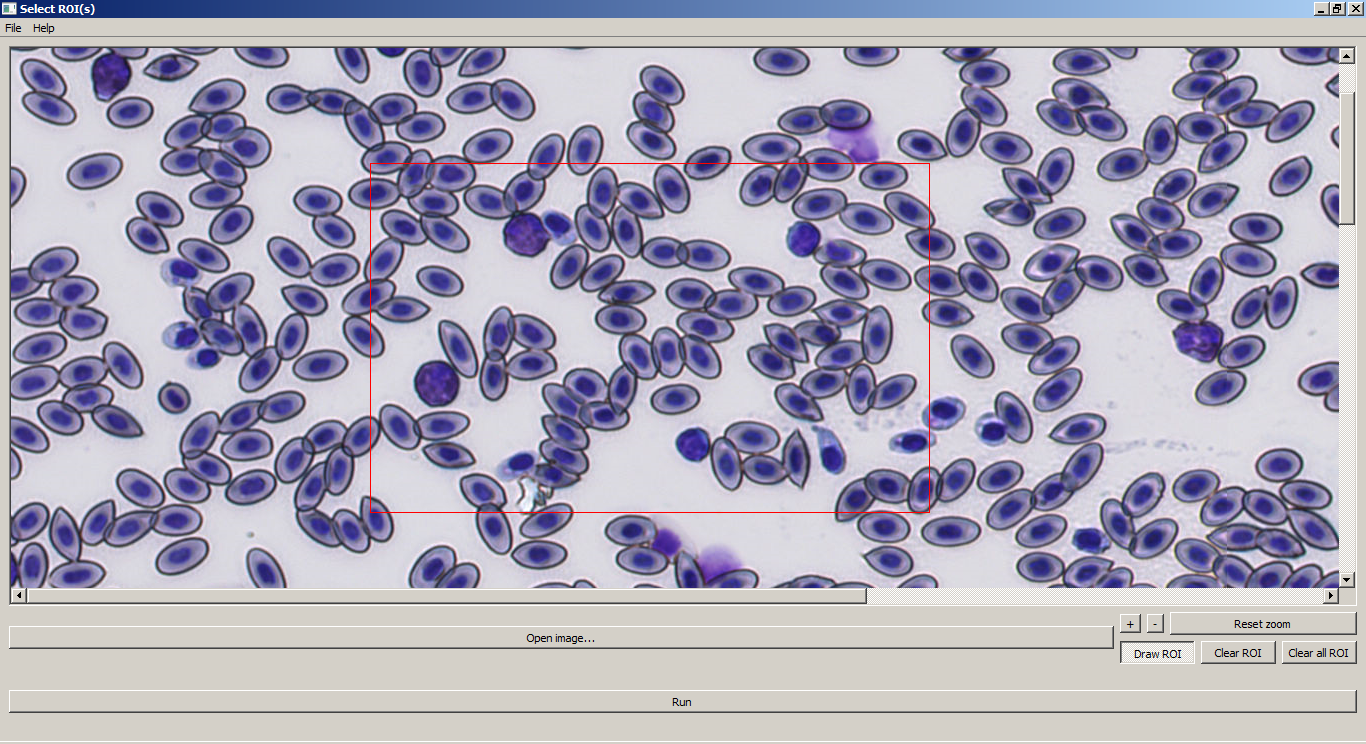
\includegraphics[width=\textwidth]{../fig/select_rois2.png}
    \caption{Simple example showing how the main window of the GUI works, with a minimal ROI selected.}
    \label{fig:select_rois}
\end{figure}

\begin{figure}[h!]
    \centering
    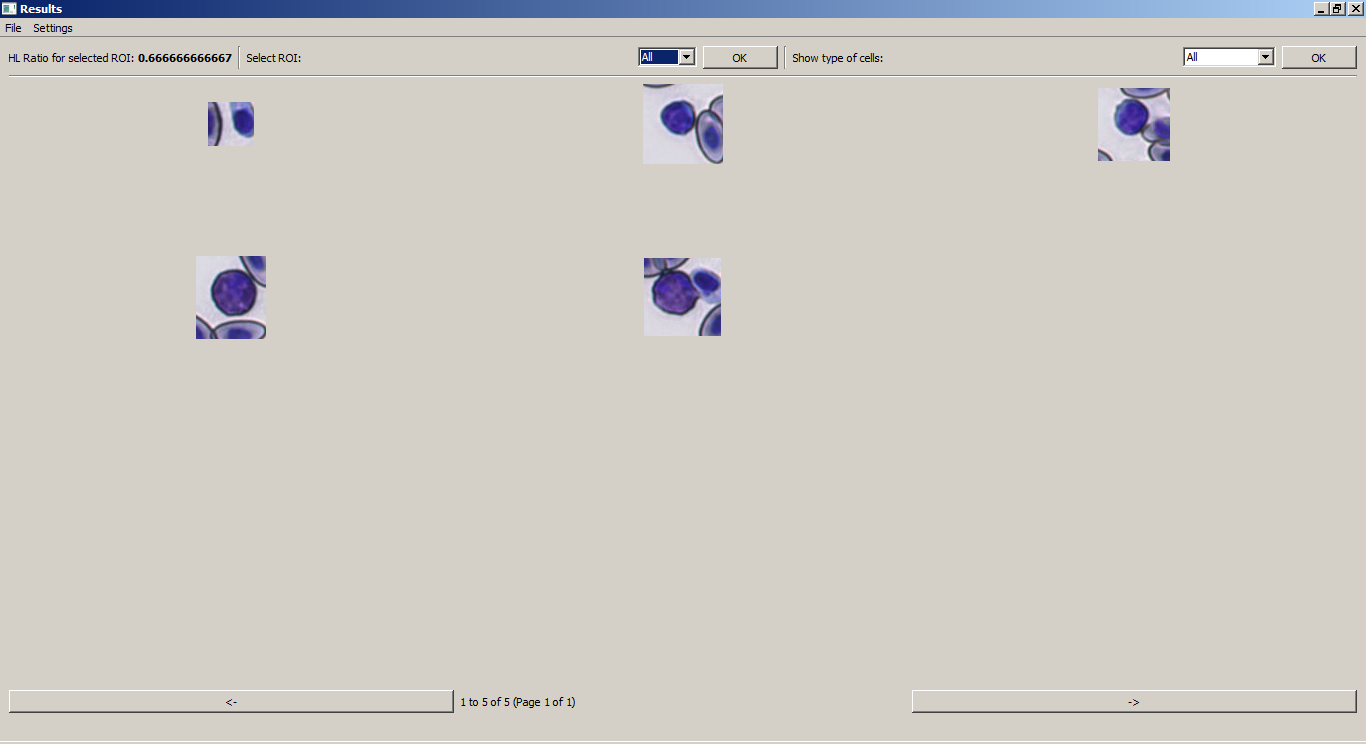
\includegraphics[width=\textwidth]{../fig/results.png}
    \caption{Results from the previous ROI, where the first cell is a probable wrongly classified red blood cell.}
    \label{fig:select_rois}
\end{figure}

\begin{figure}[h!]
    \centering
    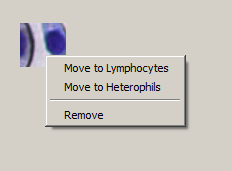
\includegraphics{../fig/moveto.png}
    \caption{Right-click menu showing the different options for removing or moving cells to another category.}
    \label{fig:select_rois}
\end{figure}


\subsection{Implementation}
The interface was implemented in Qt Creator, which is a cross-platform integrated development environment (IDE) that includes an integrated GUI layout and forms designer. This greatly reduced the implementation time since GUI design can otherwise be a tedious and time consuming activity. 

\section{Evaluation}\label{sec:research:history}
